\section{SCD}
\thispagestyle{fancy}


 \gls{SCD} (System Control Diagram) er eit grafisk dokumentasjons verktøy beskrevet i IEC PAS 63131. \newline
 \gls{SCD} blir brukt for å vise relasjonane mellom prosessens komponentar og programmet som styrer dei og skiljer seg frå eit \gls{PID}
 som dokumenterer alt fysisk utstyr.

 Vi ynskjer å bruke SCD som eit planleggingsverktøy for programstrukteren. SCD inneheld IEC templat noko som gjer at ein kan
 planlegge programmering av anlegget før ein har skreve sjølve IEC blokk-koden
 Diagrammet gir oss mulighet til å visualsere, teikne og kople IEC blokkene mot komponentane på anlegget og 
 gir oss også ein unik moglegheit for å kunne dokumentere arbeidet og vil gi ein grafisk representasjon
 av styringsform og løysningar som blir valgt.

 Vi har kontakta MIDTechology\citep{MIDT} som er som er eit selskap som utviklar programvare for SCD og har fått utlevert studentlisensar
 til programvaren. Vi vil bruke dette programmet for planlegging og dokumentering av koden til reiseanlegget på Sande.

 \begin{figure}[htbp]
    \centering
    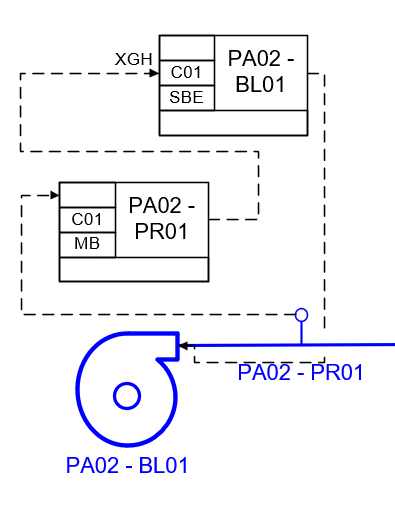
\includegraphics[width=0.35\textwidth]{Bilder/Visio_eksempel.png}
    \caption{Eksempel av SCD}\label{fig:SCD eksempel}    
\end{figure}

\newpage